\begin{figure} [H]
	\centering
	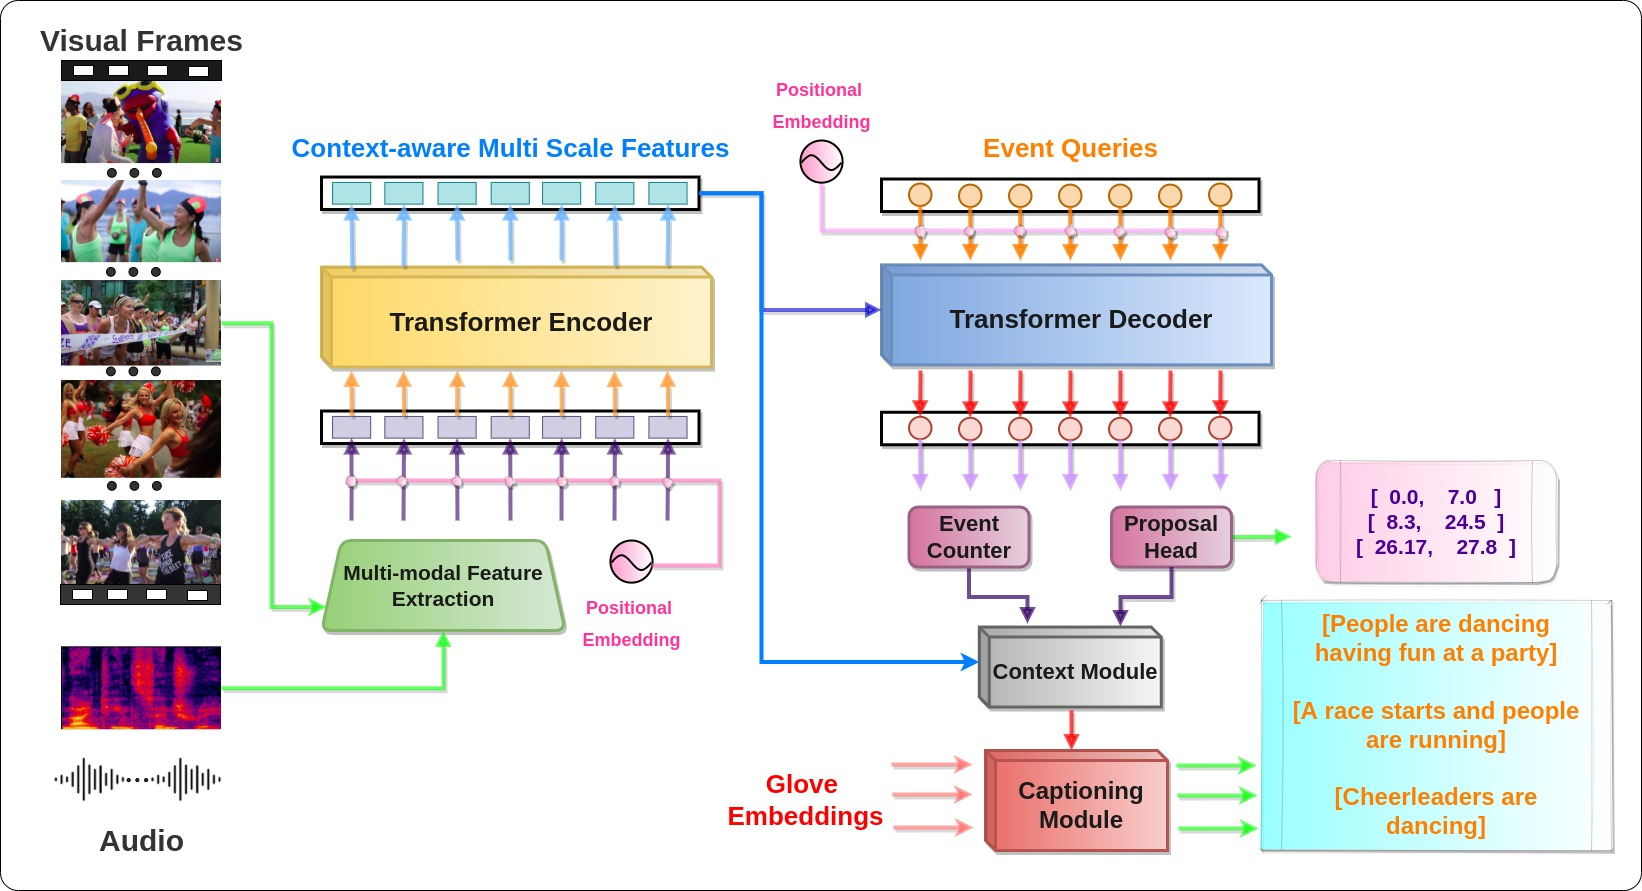
\includegraphics[width=\linewidth]{assets/img/architecture-no-bg.jpg}
	\caption{Proposed model architecture for Dense Video Captioning} %TODO add description?
\end{figure}

\section{Multimodal Feature Extraction}
\par Feature extraction is the backbone of our solution to tackle the task of Dense Video Captioning \cite{krishna2017densecaptioning}. A rich feature space would enhance the representational power of the model, thereby leading to more meaningful and accurate event proposals. Most previous works have utilized one modality only (i.e. video) to generate feature vectors as input to the proposal generator. However, audio cues, in conjunction with video frames is a strong event indicator. These events are accompanied with sharp changes in their corresponding audio spectrograms which can be learnt by the model to better determine the precise boundary of events. Thus, we aim to combine features generated using both video and audio. For this, we pre-train our encoders using the Temporally Sensitive Pre-training \cite{alwassel2021tsp} paradigm which is further explained in Chapter \ref{chapter:feat}.


\section{Proposal Generation}
\par Proposal generation is at the core of the dense video captioning task. It predicts the start and end time of events in the video which would then be used for captioning. Most previous works have used CNN-based architectures to predict event timestamps, but require a lot of fine-tuning to achieve competitive results.
\par We use an encoder-decoder architecture proposed by \cite{carion2020detr} and adapt it to work with videos across multiple modalities. Moreover, we implement deformable  attention \cite{zhu2020deformable} with token sparsification \cite{roh2021sparse} to decrease the quadratic time complexity of regular attention and improve event localization.
\par For all our losses, we assume $y$ as ground-truth events and $\hat{y}=\left \{ \hat{y_{i}} \right \}_{i=0}^{N}$ as the model predictions, where $N$ is the number of events in a batch.

\subsection{Transformer Encoder}
\par The transformer encoder consists of a deformable, multi-headed self-attention module followed by a feed-forward neural network (FFN). 
\par The encoder receives as input, multi-scale features $x_{0} \in R^{(N , d)}$ for $l$ feature levels, $N = \sum_{i=0}^{l-1}\left \{\frac{n}{i} \right \}$, where $d$ is the dimension of the model . The output of the encoder $m_{0} \in R^{(N , d)}$ belongs to a richer feature space tailored specifically for event localization and is treated as \textit{video memory} for the decoder. We also add fixed positional embeddings to each feature level of the input to overcome the permutation-invariance of transformers. 
\par We also use auxiliary loss (discussed in \ref{chapter:aux}) for all layers of the encoder except the last, which is used exclusively as input to the decoder.

\subsection{Transformer Decoder}
The transformer decoder consists of multi-headed self-attention and cross-attention modules (which can either follow the deformable or sparse attention paradigms) followed by a feed-forward neural network (FFN). The input to the decoder $q_{0} \in R^{(Q , d)}$ consists of $Q$ different embeddings, each representing a particular event in the video. Analogous to \cite{carion2020detr}, these $Q$ embeddings are learnt positional embeddings or \textit{event queries} and are added to the input (similar to the encoder). The decoder attends the \textit{event queries} with the \textit{video memory} and outputs embeddings $z_{0} \in R^{(Q , d)}$.
\par The output of the decoder is the fed to two prediction heads, namely the \textit{segment head} and the \textit{event counter}. The \textit{segment head} is a 3-layer FFN with the GELU activation function and and output dimension of 2, representing the normalized center-offset and length for an event. We calculate 2 losses for event segments, namely the $l1$ loss and the generalized $IoU$ (Intersection over Union) loss, normalized by the number of event segments in the batch.

$$\L_{l1} =  \left \| b_{i} - \hat{b_{i}} \right \| \hspace{1cm} \L_{giou} = \frac{\left |C\symbol{92}(A\cup B)   \right |}{\left | C \right |} $$

\par The \textit{event counter} consists of a single linear layer with an output dimension equaling the maximum predicted events in a video. Next, we use the $argmax$ function to find the $N_{set}$ followed by selecting the top-k events from the $N_{set}$ based on these confidence scores. We then calculate the cross-entropy loss $\L_{event}$ between the predicted, high-confidence event counts and the ground-truth event counts.

\subsection{Attention}
\par The attention mechanism proposed in \cite{tfm} has quadratic complexity as each token attends to every other token in the sequence. This may be important for text, but for images and videos (especially for the dense video captioning task), attending to a smaller set of tokens in a concentrated area is sufficient and can greatly reduce the time complexity. 
We implement deformable attention \cite{zhu2020deformable}, which attends to only a small set of key sampling points around a reference point, regardless of the spatial
size of the feature maps. Given an input feature map $x \in R^{C\times H \times W}$ , let q index a query element with content feature $z_q$ and a 2-d reference point $p_q$, the deformable attention feature is calculated by
$$ DeformAttn(z_q, p_q, x) = \displaystyle\sum\limits_{m=1}^M W_m
[\displaystyle\sum\limits_{k=1}^K A_{mqk}\cdot W'_mx(p_q+\Delta p_{mqk})]
$$
\par where k indexes the sampled keys, m indexes the attention head, and K is the total sampled key number. $\Delta p_{mqk}$ and $A_{mqk}$ denote the sampling offset and attention weight of the $k^{th}$ sampling point in the $m^{th}$ attention head, respectively.
\par Deformable attention module can be easily extended for multi-scale feature maps. Let $\{{x^l}\}_{l=1}^L$ be the input multi-scale feature maps, where  $x^l \in R^{C\times H^l \times W^l}$ . Let $ \hat p_q \in [0, 1]^2$ be the normalized coordinates of the reference point for each query element q, then the multi-scale deformable attention module is applied as

$$DeformAttn(z_q, \hat{p}_q, \{{x^l}\}_{l=1}^L) = 
\displaystyle\sum\limits_{m=1}^M W_m
[\displaystyle\sum\limits_{l=1}^L\displaystyle\sum\limits_{k=1}^K A_{mlqk}\cdot W'_mx^l(\phi _l (\hat p_q)+\Delta p_{mlqk})]$$

\par where l indexes the input feature level, m indexes the attention head, and k indexes the sampling point. $\Delta p_{mlqk}$ and $A_{mlqk}$ denote the sampling offset and attention weight of the $k^{th}$ sampling point in the $l^{th}$ feature level and the $m^{th}$ attention head, respectively

\par We further reduce the encoder tokens that should be further modified on the fly by
predicting a pseudo-ground truth of the saliency defined by decoder cross-attention maps \cite{roh2021sparse}.
The saliency of each input token is determined by aggregating the decoder cross-attentions between all \textit{event queries} and the encoder output. It generates a single map of the same size as the backbone’s feature map, which is known as the Decoder cross Attention Map (DAM). To train the scoring network, we binarize DAM so that only the top-k percentage of encoder tokens are
kept. To predict how likely a given encoder token is to be included in the top-p\% most referenced tokens, a 4-layer scoring network g is used, and the network is trained by minimizing the binary cross entropy (BCE) loss between the binarized DAM and prediction.

$$\L_{dam} = -\frac{1}{N}\displaystyle\sum\limits_{i=1}^N BCE(g(X_{feat})_i, DAM^{bin}_i)$$


\section{Context Mask Module}
\par Once the decoder predicts the events, we consider only those features of the video that belong to those particular events. For this, we use a differentiable masking network proposed by \cite{zhou2018end} instead of static masks used by most previous works.
\par The network is a simple FFN with an output dimension of $N=video sequence length$. It gets as input, normalized center offsets and lengths from the segment head and outputs a differentiable mask with values (near) zero when outside the event segments, and (near) one otherwise. Then, we perform an element-wise product with the \textit{video memory} produced by the encoder and feeds this output to the captioning module.
\par We use the Binary Cross-Entropy loss function between the binary (static) mask made using predicted event boundaries and the differentiable mask.

$$\L_{m} = \textrm{BCE}(\mathit{Bin}(S_{p}, E_{p}), f_{FFN}(S_{p}, E_{p}))$$

\section{Captioning Module}
\par We use the transformer decoder proposed by \cite{tfm} along with 300-dimensional GloVe word embeddings pre-trained on 6 billion tokens\cite{glove}. The word embeddings are attended with the \textit{video memory} and output embeddings are fed into a softmax layer over the entire vocabulary to get next-word probabilities.
\par We use the KL divergence loss along with label smoothing to encourage small logit gaps and prevent the model from being too confident about its predictions.

$$y _{c}= (1 - \alpha)y_{onehot} + \frac{\alpha}{K} \hspace{1cm} \L_{cap}(y, \hat{y}) = \sum_{c=1}^{N}\hat{y} \log{\frac{\hat{y}}{y_c}}$$

\par where $K$ is the number of label classes, and $\alpha$ is a hyperparameter that determines the amount of smoothing.

\section{Event Set Prediction}
\par The output of the decoder consists of $Q$ event queries, each of which represents an event in the video with varying levels of confidence. $Q$ can be set based on the task complexities. Tasks such as object detection in images can have much more queries as compared to temporal action localization. The Hungarian matching algorithm \cite{hungarian} is used to suppress incorrectly assigned predicted segments to ground-truth instances when the decoder produces false positives or false negatives. We thus use a one-to-one mapping between the 2 sets and find only those assignments with the least cost (weighted bipartite matching).
\par We first calculating a cost matrix of each predicted segment against each ground truth segment. This cost is a linear combination of the $l1$ loss and the generalized $IoU$ loss.
$$ C = \alpha_{l1}\L_{l1}  + \alpha_{giou}\L_{giou}$$
\par Then, we use the Hungarian algorithm to optimally match predicted and ground truth segments by selecting the mappings with the lowest cost. Finally, we calculate the overall Hungarian loss across all selected segments for backpropagation through the entire model.

$$\L_{Hungarian}(y, \hat{y}) = \sum_{i=0}^{N}\left [ \alpha_{l1}\L_{l1} + \alpha_{giou}\L_{giou} + \alpha_{event}\L_{event} + \alpha_{m}\L_{m} + \alpha_{cap}\L_{cap} \right ]$$

\section{Auxiliary Losses} \label{chapter:aux}
\par To mitigate the problem of vanishing gradients and aid better learning throughput out the model, we utilize auxiliary losses during training for the transformer encoder, decoder and captioning module. We thus calculate the loss and backpropagate gradients for every layer of the model, just as we do for the final layer. However, we do not calculate the context mask loss as it is too expensive and requires more training time.
\par \cite{carion2020detr} does not calculate auxiliary loss for the encoder as its tokens are significantly more in number as compared to the decoder's tokens. However, due to sparsification from the decoder attention map, we can calculate the auxiliary loss for each layer in the encoder, but only for the selected tokens. 

\subsection{Gradient Flow}

\par Gradients and its flow is always a issue when dealing with large and complex models. With models based on the DETR \cite{carion2020detr} architecture, vanishing gradients is a problem. As suggested in \ref{chapter:aux}, we use auxiliary loss in the encoder as well. If we adopt the architecutre proposed in \cite{zhu2020deformable}, with no auxiliary loss for the encoder, the gradients through the encoder decrease at a rapid rate which in turn, reduces the rate at which the loss decreases. 
\par By using sparsification of encoder tokens and auxiliary loss across all layers of the encoder (except the last) as proposed in \cite{roh2021sparse}, the gradients do not vanish and are much more uniform across the entire model.

\begin{figure}[h]
	\centering
	\begin{subfigure}[b]{0.55\textwidth}
		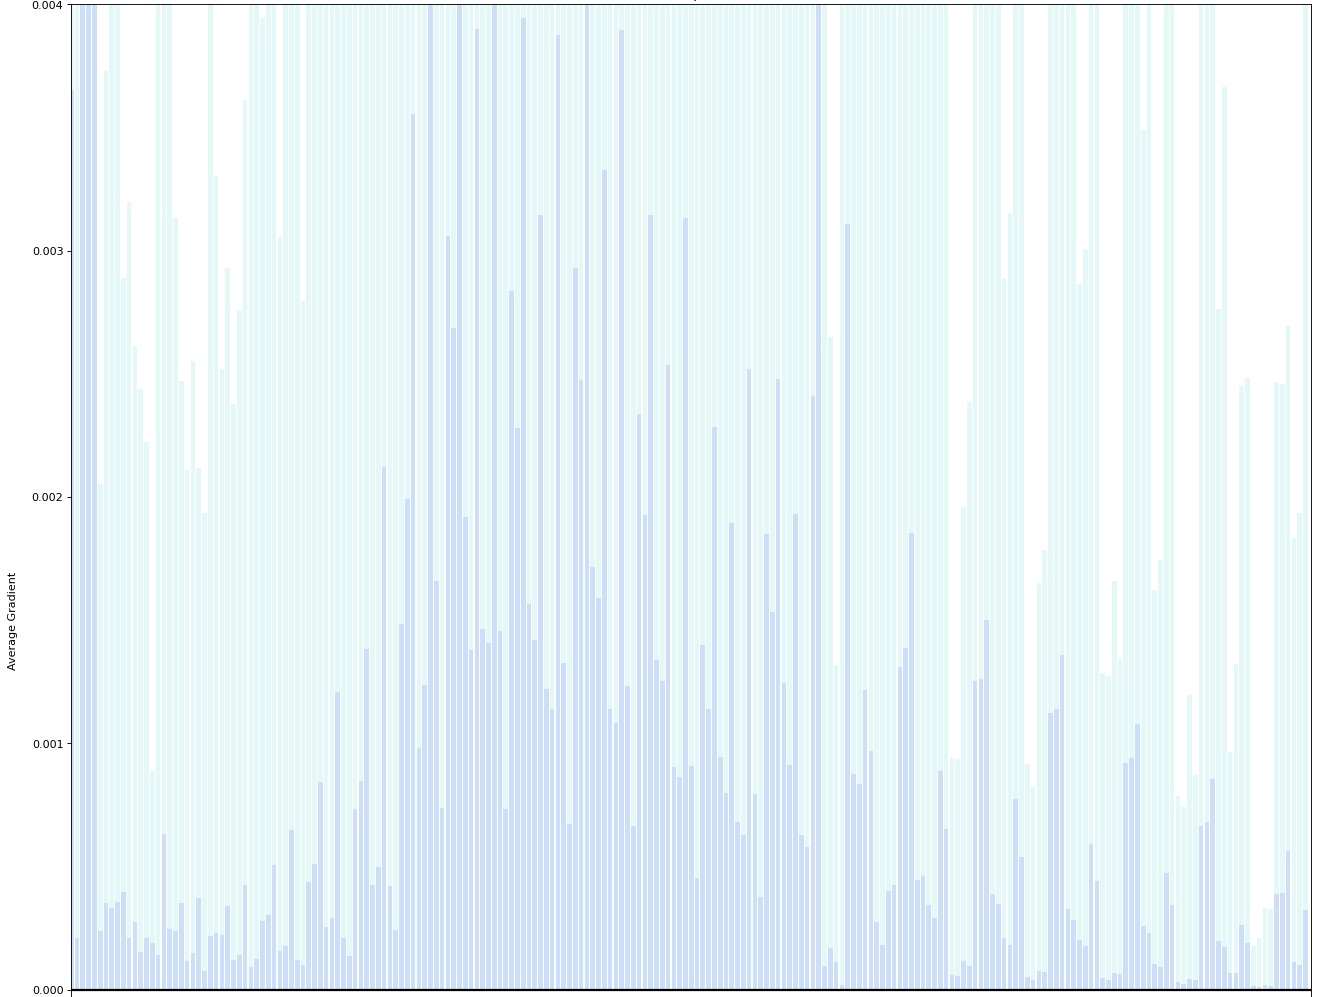
\includegraphics[width=\linewidth]{assets/img/deformable_grad_flow_epoch_1.png}
	\end{subfigure}%
	\begin{subfigure}[b]{0.55\textwidth}
		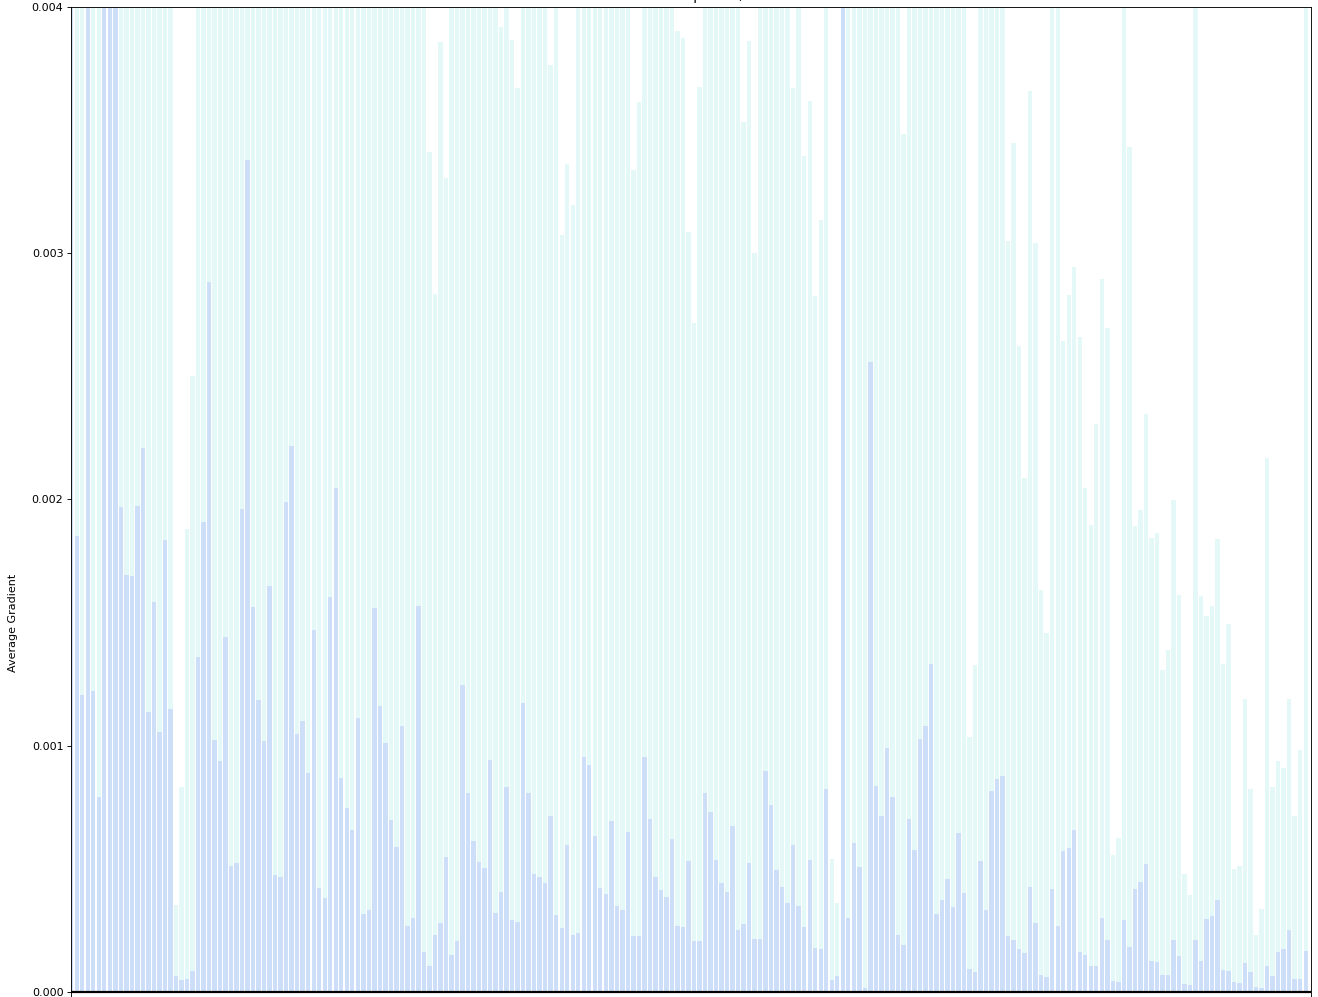
\includegraphics[width=\linewidth]{assets/img/sparse_grad_flow_epoch_1.png}
	\end{subfigure}
	\caption{Gradient flow for epoch 1 (i). Deformable Transformer, (ii). Sparse Transformer}
	
	\label{fig:gradientflowepoch1}
\end{figure}

\begin{figure}[h]
	\centering
	\begin{subfigure}[b]{0.55\textwidth}
		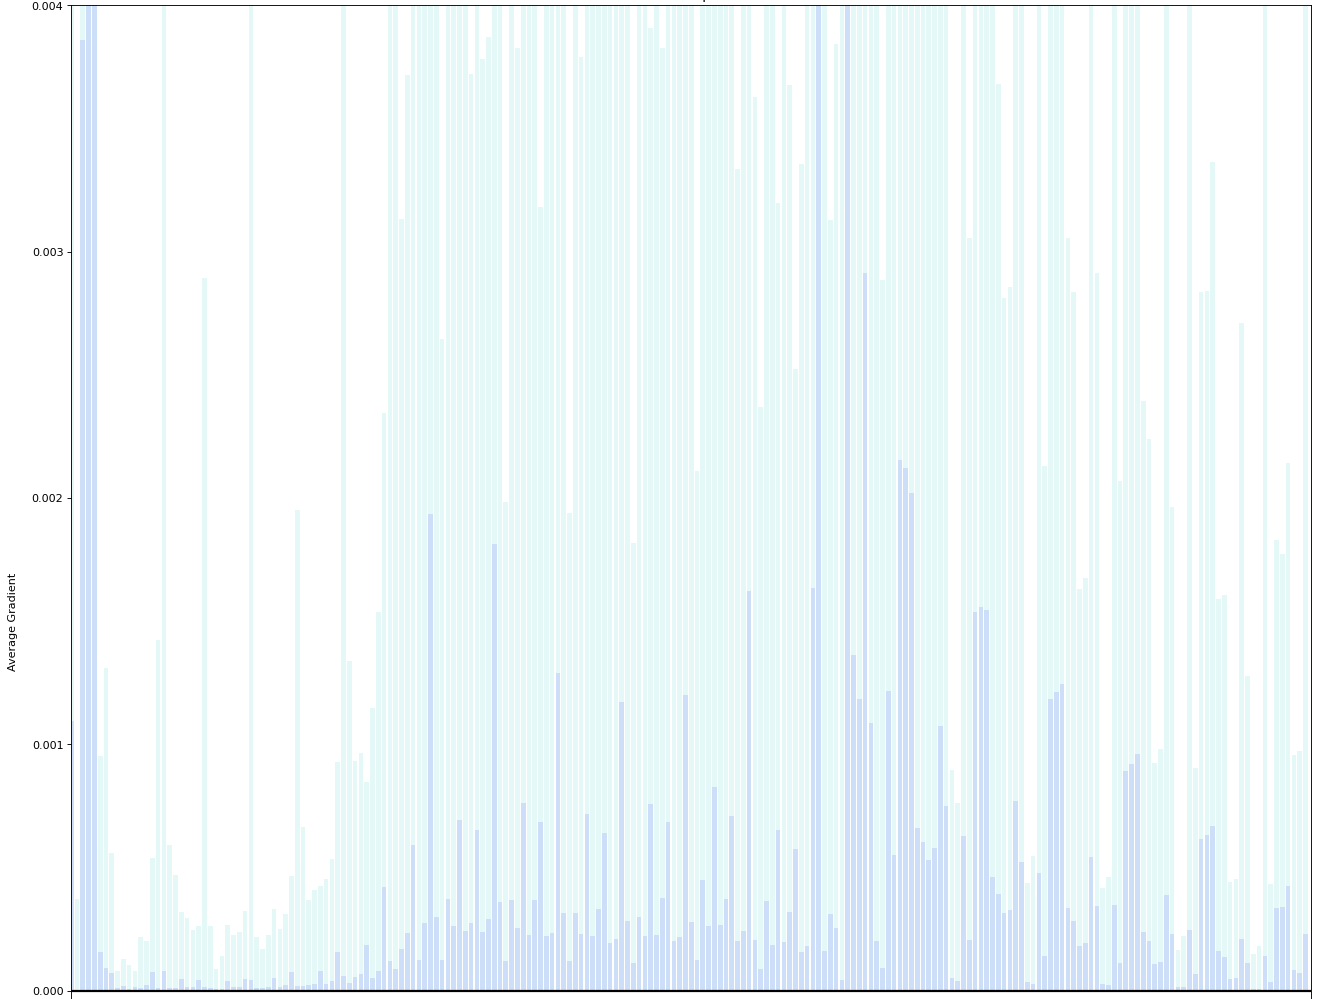
\includegraphics[width=\linewidth]{assets/img/deformable_grad_flow_epoch_8.png}
	\end{subfigure}%
	\begin{subfigure}[b]{0.55\textwidth}
		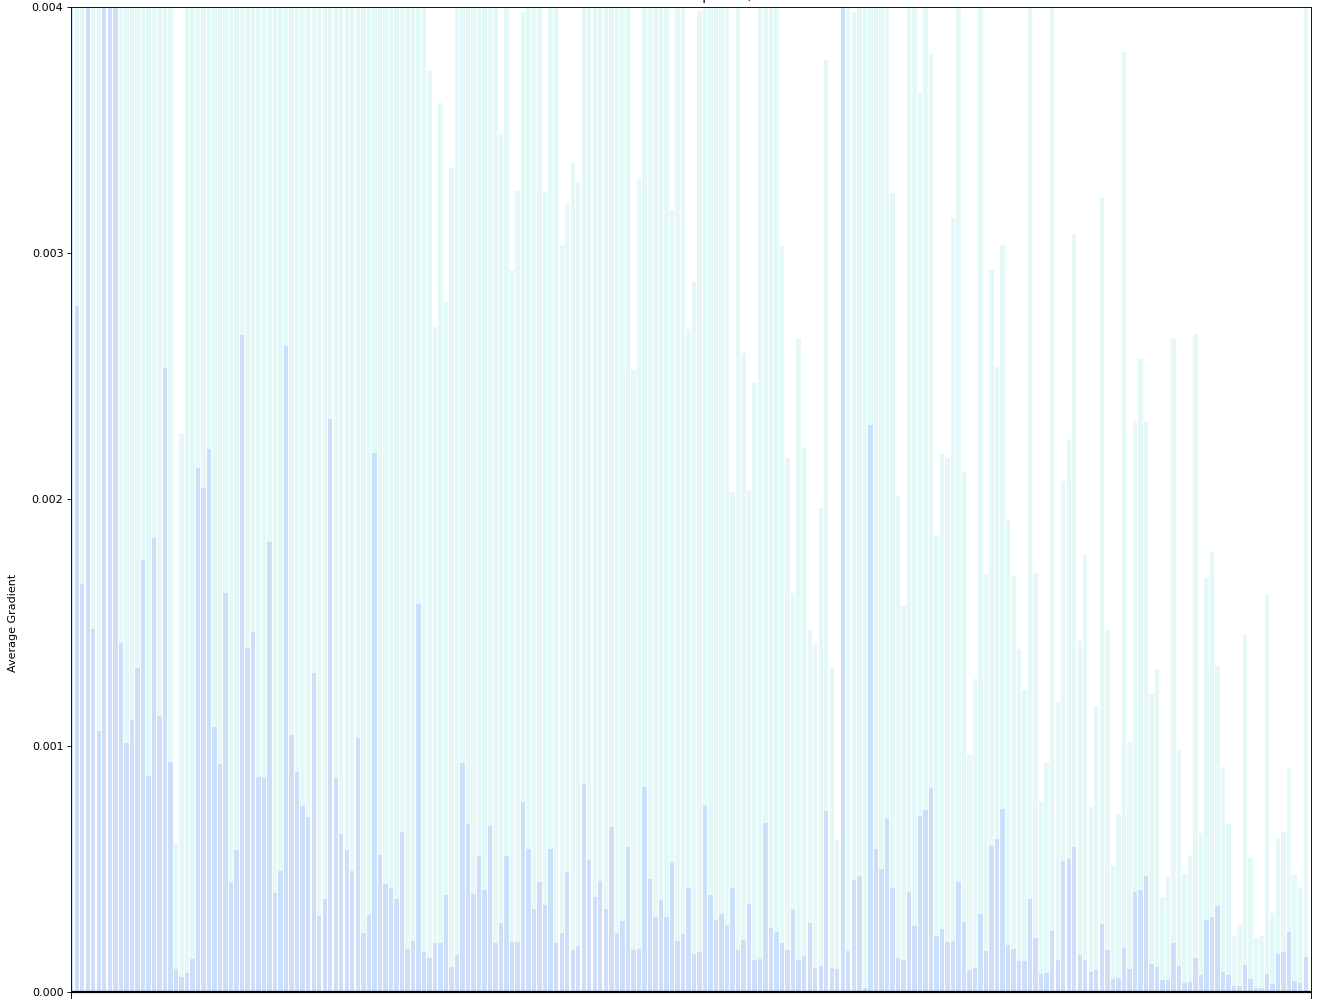
\includegraphics[width=\linewidth]{assets/img/sparse_grad_flow_epoch_8.png}
	\end{subfigure}
	\caption{Gradient flow for epoch 8 (i). Deformable Transformer, (ii). Sparse Transformer}
	
	\label{fig:gradientflowepoch8}
\end{figure}





